\section{Применение}\label{sec:ch1/application}

Рассмотренные в предыдущих разделах методы бинарной классификации позволяют успешно решать задачи разделения двух классов на компакте признакового пространства. В данном разделе рассматриваются примеры, иллюстрирующие особенности работы моделей, использующих описанную в разделе~\cref{subsec:ch1/bayesian_classifier_modification} модификацию, а также проблемы, которые такая модификация позволяет эффективно решать.

%%%%%%%%%%%%%%%%%%%%%%%%%%%%%%%%%%%%%%%%%%%%%%%%%%%%%%%%%%%%%%%%%%%%%%%%%%%%%%%%%%%%%%%%%%%%%%%%%%%%%%%%%%%%%%%
\subsection{Поведение вне носителя распределения}

Обычные бинарные классификаторы, обученные по конечной выборке без дополнительного ``фона``, склонны выдавать уверенные предсказания даже в тех точках пространства, где отсутствуют обучающие данные. Это поведение связано с тем, что модель не знает о структуре плотности признаков и минимизирует ошибку лишь на ограниченном множестве точек.

Рассмотрим демонстрационный пример с двумя классами, заданными в виде спиралей на двумерной плоскости. На рисунке~\cref{fig:spirals_example}\subcaptionref{fig:spirals_example_classic} представлено решение, полученное обычным бинарным классификатором. Видно, что модель уверенно относит к одному из классов даже точки, расположенные далеко за пределами области, покрытой обучающими данными.

Для сравнения, если использовать, описанную в разделе~\cref{subsec:ch1/neural_approximation} модифицированную процедуру, то классификатор начинает учитывать общую структуру распределения данных и классифицирует ``внешние`` точки как фон (рисунок~\cref{fig:spirals_example}\subcaptionref{fig:spirals_example_modified}). Это значительно повышает надёжность предсказаний и позволяет говорить о появлении эффекта отказа от распознавания вне носителя распределения.

\begin{figure}[ht]
    \centerfloat{
        \hfill
        \subcaptionbox{классический классификатор\label{fig:spirals_example_classic}}{%
            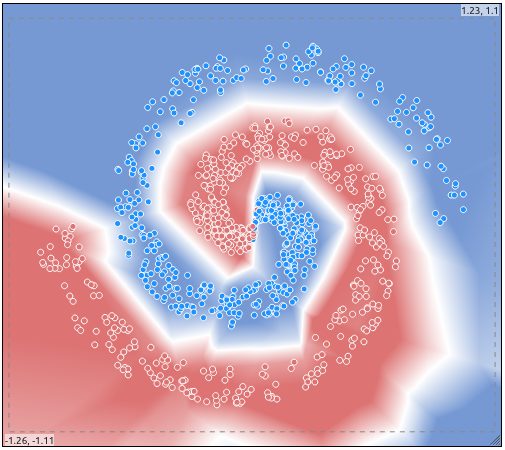
\includegraphics[width=0.48\linewidth]{Dissertation/images/ch1/application/spirals_usual.png}}
        \hfill
        \subcaptionbox{модифицированный классификатор\label{fig:spirals_example_modified}}{%
            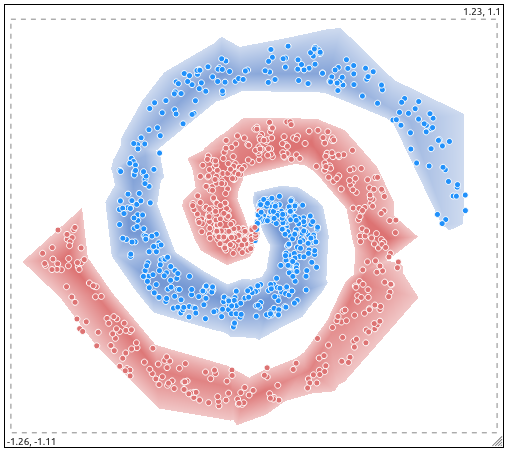
\includegraphics[width=0.48\linewidth]{Dissertation/images/ch1/application/spirals_modified.png}}
        \hfill
    }
    \caption{Сравнение поведения классификаторов вне носителя}
    \label{fig:spirals_example}
\end{figure}

%%%%%%%%%%%%%%%%%%%%%%%%%%%%%%%%%%%%%%%%%%%%%%%%%%%%%%%%%%%%%%%%%%%%%%%%%%%%%%%%%%%%%%%%%%%%%%%%%%%%%%%%%%%%%%%
\subsection{Устойчивость}

Модели, обучаемые без использования фона, оказываются чрезвычайно чувствительными к отдельным аномальным точкам. Добавление даже одной точки может радикально изменить форму решающего правила (рисунок~\cref{fig:backdor_attack}\subcaptionref{fig:backdor_attack_classic}). Это явление лежит в основе так называемых backdoor-атак~\cite{guo2022overview}, когда намеренно добавленные в обучающую выборку точки провоцируют нежелательное поведение модели в заранее заданной области.

Добавление фона значительно снижает эффект подобных атак (рисунок~\cref{fig:backdor_attack}\subcaptionref{fig:backdor_attack_modified}). Чтобы в присутствии фона точка начала влиять на решение, необходимо существенно увеличить её плотность, что требует добавления множества подобных примеров. Таким образом, обучение с фоном повышает устойчивость модели к целевым модификациям данных.

\begin{figure}[ht]
    \centerfloat{
        \hfill
        \subcaptionbox{классический классификатор\label{fig:backdor_attack_classic}}{%
            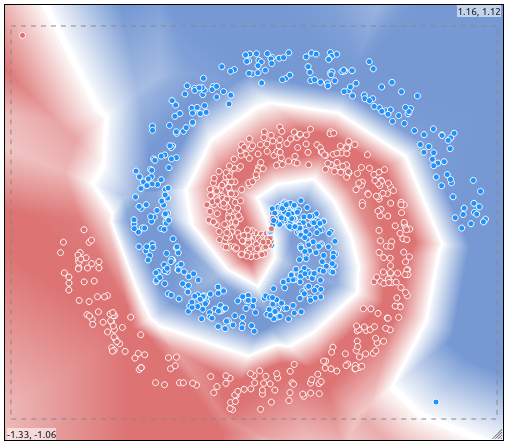
\includegraphics[width=0.48\linewidth]{Dissertation/images/ch1/application/backdor_usual.png}}
        \hfill
        \subcaptionbox{модифицированный классификатор\label{fig:backdor_attack_modified}}{%
            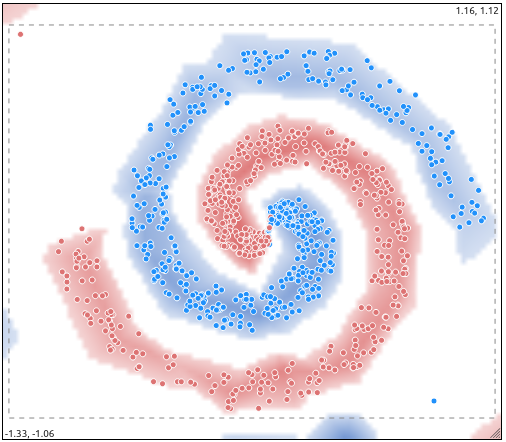
\includegraphics[width=0.48\linewidth]{Dissertation/images/ch1/application/backdor_modified.png}}
        \hfill
    }
    \caption{Сравнение устойчивости классификаторов к backdoor-атаке}
    \label{fig:backdor_attack}
\end{figure}

%%%%%%%%%%%%%%%%%%%%%%%%%%%%%%%%%%%%%%%%%%%%%%%%%%%%%%%%%%%%%%%%%%%%%%%%%%%%%%%%%%%%%%%%%%%%%%%%%%%%%%%%%%%%%%%
\subsection{Противодействие SLAP атаке}

Одним из наиболее уязвимых мест классических классификаторов является их поведение на границе принятия решений. Это свойство активно используется в рамках предложенной в разделе~\cref{sec:ch1/slap} атаки SLAP.

Модифицированная процедура классификации, использующая фоновый класс, существенно снижает эффективность подобного рода атак. На рисунке~\cref{fig:slap_modified_attack} представлены примеры атак, полученных с использованием метода SLAP как для классической модели, так и для модели с фоном. При этом использование модифицированной процедуры обучения приводит к следующим эффектам:

\begin{itemize}
  \item во многих случаях атака не удаётся;
  \item при отсутствии ограничений на допустимую область признаков атакующие точки часто выходят за пределы компакта, что приводит к отказу от их распознаванию;
  \item при успешной атаке полученные точки, как правило, попадают в области с низким уровнем доверия, что также приводит к отказу от распознавания.
\end{itemize}

Таким образом, модификация классификатора с введением фонового класса позволяет эффективно нейтрализовать атаку SLAP, построенную без использования градиентной информации и не зависящую от конкретной архитектуры модели.

%%%%%%%%%%%%%%%%%%%%%%%%%%%%%%%%%%%%%%%%%%%%%%%%%%%%%%%%%%%%%%%%%%%%%%%%%%%%%%%%%%%%%%%%%%%%%%%%%%%%%%%%%%%%%%%
\subsection{Сопоставление нейросетевой и гистограммной регрессии}

В разделе~\cref{subsec:ch1/histogram_approximation} рассматривалось иерархическое разбиение компакта нейросетевой моделью на ячейки, на основе которых строилась функция гистограммной регрессии. Визуальное сопоставление результатов нейросетевой и гистограммной регрессий подтверждает близость этих методов: выход нейросети в силу своей непрерывности плавно переходит от одного класса к другому, приближая собой ступенчатую структуру гистограммы (рисунок~\cref{fig:cn_vs_hn}). Ячейки гистограммы, на которые разбивает пространство персептрон, окрашены в соответствии со значением \(h_n^*(X)\) в ячейке и визуально очень похожи на выход нейросети.

Это наблюдение позволяет рассматривать регрессию на выходе многослойного персептрона как мягкую версию гистограммной аппроксимации, реализуемую при помощи кусочно-линейных функций.

\begin{figure}[ht]
    \centerfloat{
        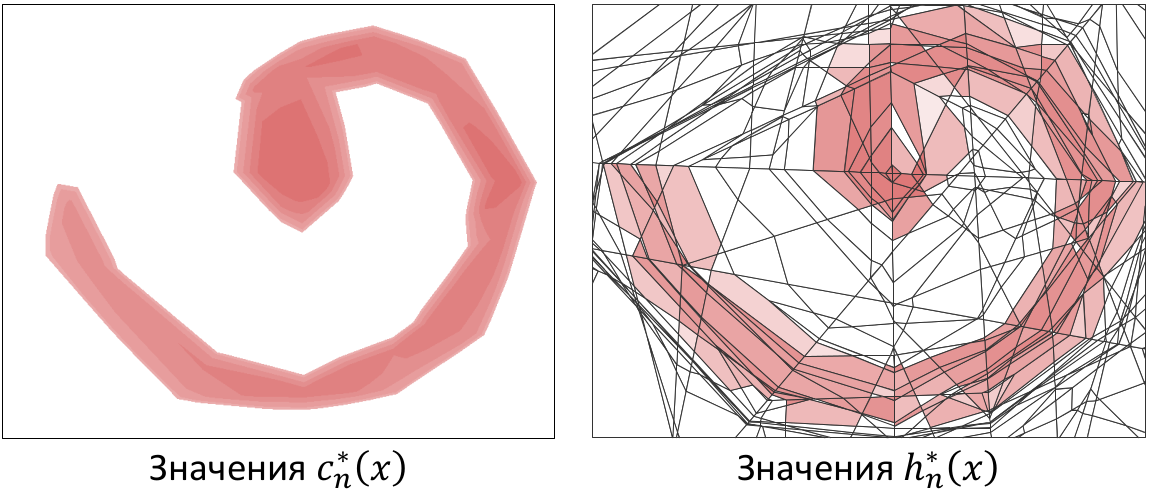
\includegraphics[width=0.9\linewidth]{Dissertation/images/ch1/application/cn_vs_hn.png}
    }
    \caption{Визуальное сравнение функций нейросетевой и гистограммной регрессий}
    \label{fig:cn_vs_hn}
\end{figure}

%%%%%%%%%%%%%%%%%%%%%%%%%%%%%%%%%%%%%%%%%%%%%%%%%%%%%%%%%%%%%%%%%%%%%%%%%%%%%%%%%%%%%%%%%%%%%%%%%%%%%%%%%%%%%%%
\subsection{Отказ от распознавания и интерпретация выходов}

Добавление фона позволяет не только лучше моделировать границу классов, но и реализовать механизм отказа от распознавания: наблюдения, попадающие в области низкой плотности, классифицируются как ``неизвестные``. Это открывает путь к более гибкому принятию решений -- например, маркированию таких примеров для дополнительного анализа или анализа дополнительных признаков.

%%%%%%%%%%%%%%%%%%%%%%%%%%%%%%%%%%%%%%%%%%%%%%%%%%%%%%%%%%%%%%%%%%%%%%%%%%%%%%%%%%%%%%%%%%%%%%%%%%%%%%%%%%%%%%%
\subsection{Влияние порога доверия на характеристики классификатора}
В рамках предложенного подхода в качестве дополнительного механизма контроля за качеством классификации вводится параметр \(\beta \in [0, 1)\), интерпретируемый как порог доверия. Значение \(\beta\) используется для принятия решения о классификации наблюдения: если значение выхода модели по модулю не превышает \(\beta\), классификатор воздерживается от принятия решения, т.е. формирует отказ от распознавания.

Введение порога \(\beta\) позволяет контролировать баланс между полнотой и надёжностью классификационных решений. При низких значениях \(\beta\) классификатор склонен выдавать решения по всем поступающим наблюдениям, включая случаи с высокой неопределённостью. При этом возрастает риск ошибочной классификации, особенно вблизи границ разделяющих поверхностей. Повышение значения \(\beta\) ведёт к росту количества отказов от распознавания, но одновременно повышает достоверность решений по тем наблюдениям, для которых классификация всё же производится.

На рисунке~\cref{fig:beta_thresholds} приведена визуализация результатов классификации при различных значениях порога \(\beta\): от 0 (классификация осуществляется по всем наблюдениям) до 0.5 (классификатор выдаёт решение только в случаях высокой уверенности). Видно, что при увеличении \(\beta\) область отказов расширяется (обозначена белым цветом), что соответствует желаемому поведению системы в условиях ограниченной уверенности модели.

\begin{figure}[ht]
    \centerfloat{
        \hfill
        \subcaptionbox{\(\beta = 0\)}{%
            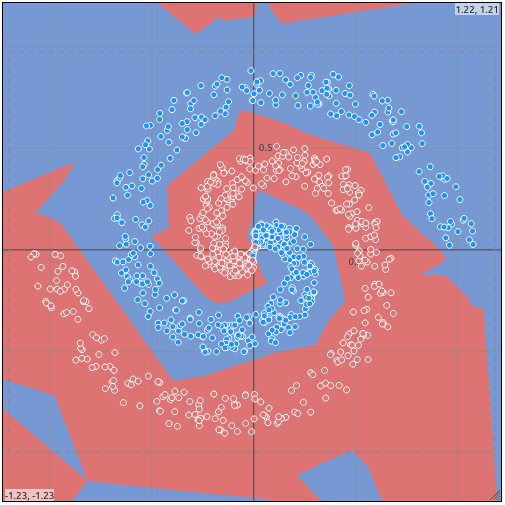
\includegraphics[width=0.24\linewidth]{Dissertation/images/ch1/application/beta0.0.png}}
        \hfill
        \subcaptionbox{\(\beta = 0.1\)}{%
            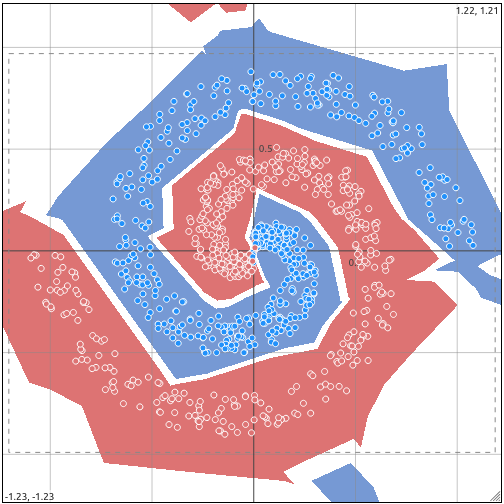
\includegraphics[width=0.24\linewidth]{Dissertation/images/ch1/application/beta0.1.png}}
        \hfill
        \subcaptionbox{\(\beta = 0.3\)}{%
            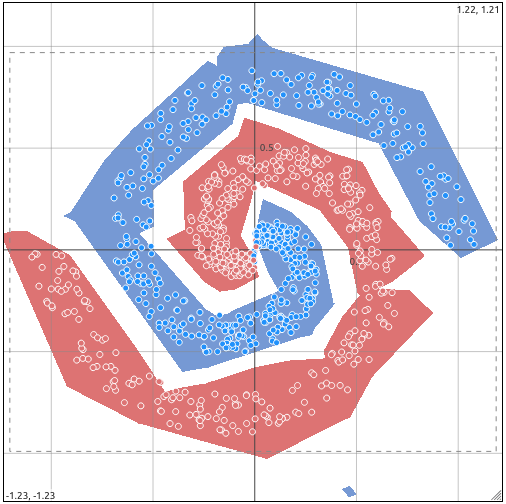
\includegraphics[width=0.24\linewidth]{Dissertation/images/ch1/application/beta0.3.png}}
        \hfill
        \subcaptionbox{\(\beta = 0.5\)}{%
            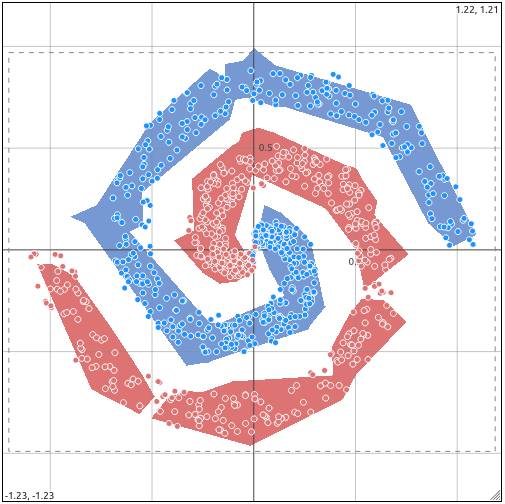
\includegraphics[width=0.24\linewidth]{Dissertation/images/ch1/application/beta0.5.png}}
        \hfill
    }
    \caption{Влияние порога доверия \(\beta\) на пространственное распределение классификационных решений}
    \label{fig:beta_thresholds}
\end{figure}

%%%%%%%%%%%%%%%%%%%%%%%%%%%%%%%%%%%%%%%%%%%%%%%%%%%%%%%%%%%%%%%%%%%%%%%%%%%%%%%%%%%%%%%%%%%%%%%%%%%%%%%%%%%%%%%
\subsection{Выводы}

Модификация бинарного классификатора позволяет существенно улучшить устойчивость и надёжность модели, основанной на многослойном персептроне. Примеры наглядно показывают, что обучение на расширенном наборе данных с добавлением фона позволяет реализовать отказ от распознавания вне носителя данных, повысить устойчивость к некоторым видам атак, а также сделать предположение о связи между функциями нейросетевой и гистограммной регрессии.
